\documentclass[letterpaper]{article}  

\usepackage{graphicx}



\begin{document}


\title{STA511 Homework \#1}
\date{}
\author{Abbas Rizvi}
\maketitle

\begin{enumerate}

\item X is a uniform random variable $(X$ $\sim$ $U(0,1))$. The histogram is shown in Figure 1a.
\begin{figure}[h!]
\caption{Histogram of uniform random variables from 0 to 1 simulated 1000 times.}

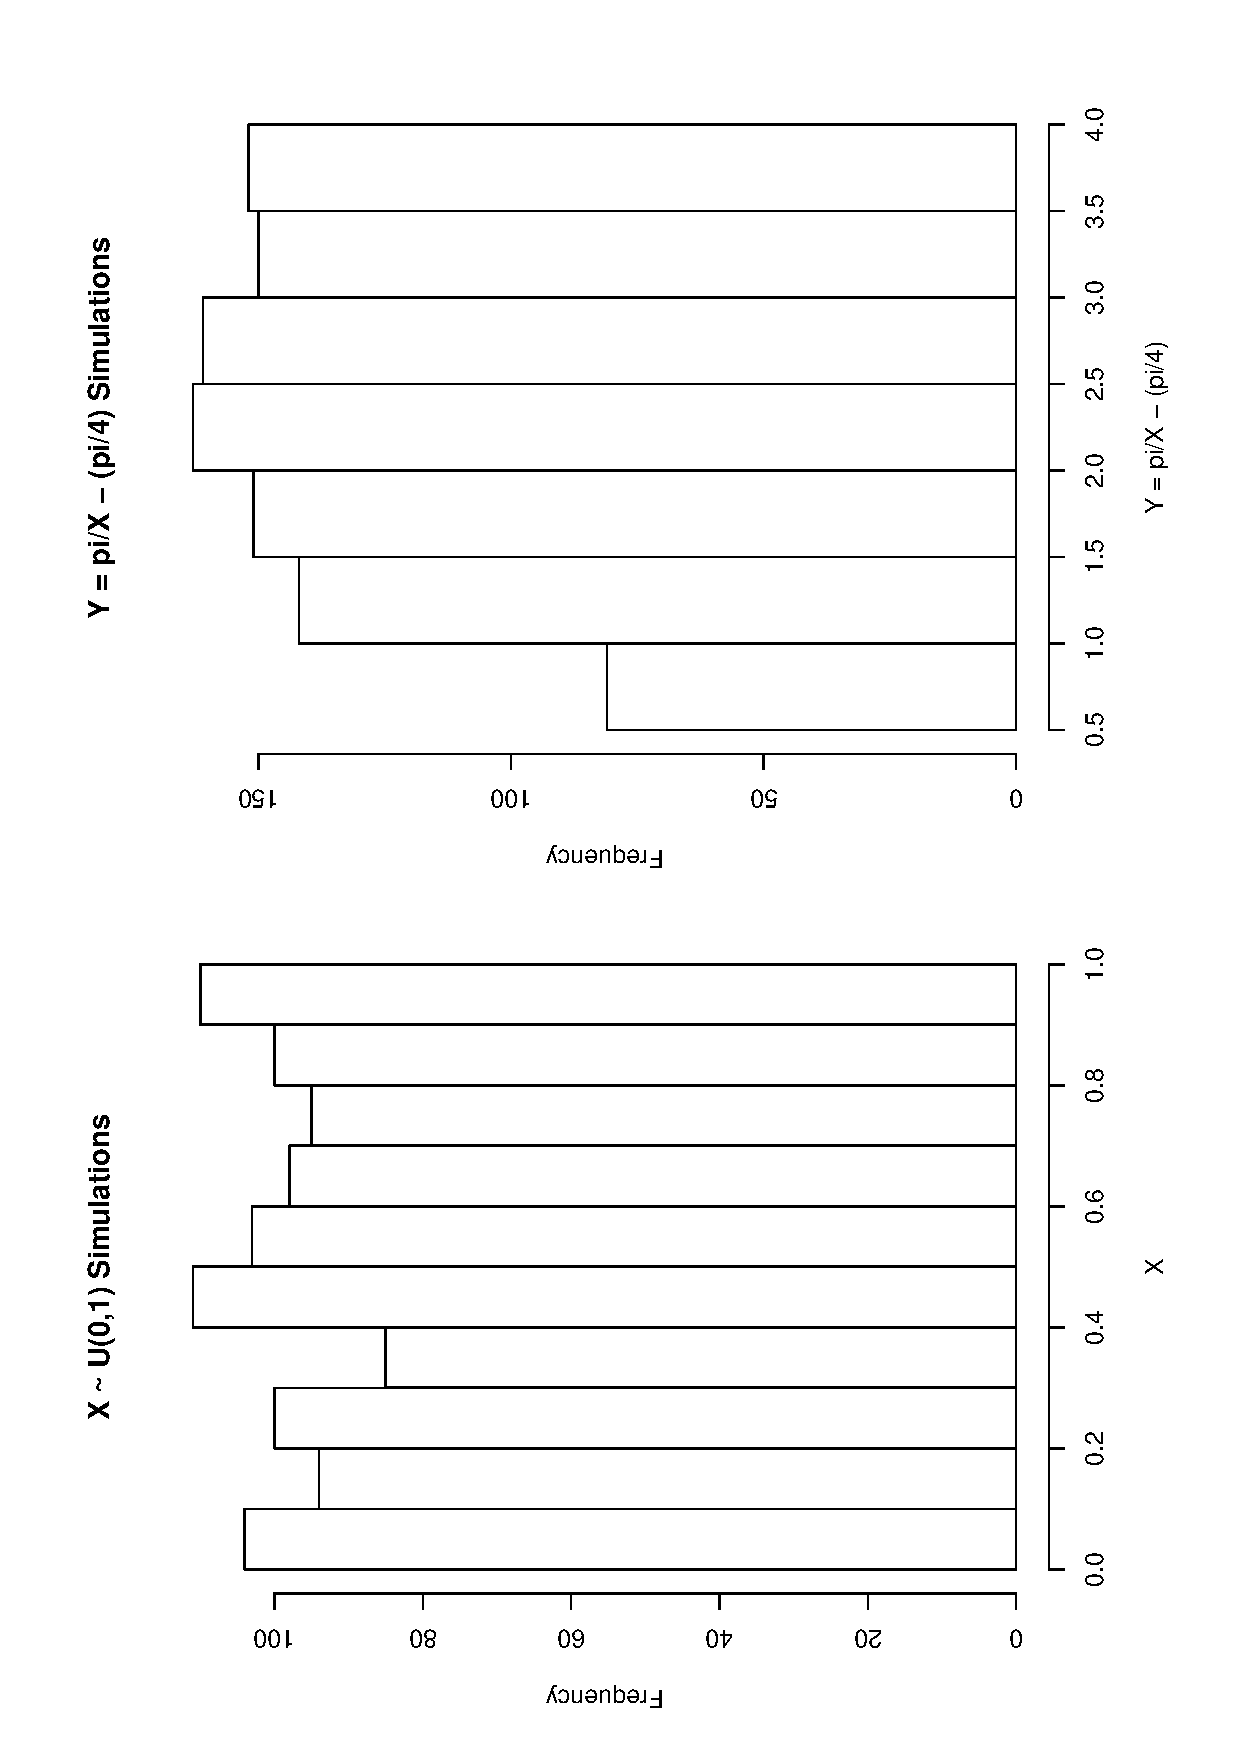
\includegraphics{hw1-q2a-runiform-histogram.pdf}
\end{figure}

\item My answer to \# 2, has multiple parts.

\begin{enumerate}
\item Here how I answered part a.
\item Here's my code for part b
\begin{verbatim}
x = rnorm(10)
hist(x)
\end{verbatim}
\end{enumerate} 

\item Ugh, this problem involves the table below
\begin{center}
\begin{tabular}{rl}
Range & Grade \\
\hline
$\geq 95$ & A\\
$\geq 90$ and $<95$ & A-\\
$\geq 85$ and $<90$ & B+\\
$\geq 80$ and $<85$ & B\\
$\geq 75$ and $<80$ & B-\\
$<75$ & C\\
\end{tabular}
\end{center}

\end{enumerate}

\end{document}
